
\section{Implementaci�n}
Con la fase de dise�o finalizada, se procede a realizar la fase de implementaci�n. Durante esta fase se genera el c�digo de la aplicaci�n y se genera el manual de usuario.

La aplicaci�n fue desarrollada en el lenguaje Java version 1.8. Con el fin de crear las interfaces de usuario se utilizo el Framework JavaFX.

En el cuadro~\ref{fig:actualizacion_implementacion} se presenta las tareas realizadas durante esta fase del desarrollo del software.

\begin{longtable}{||c| m{10cm}||}
  \caption{Actividades fase de implementaci�n}
  \label{fig:actualizacion_implementacion}
  \endfirsthead
  \hline
  N� Iteraci�n & Descripci�n\\ [0.5ex] 
  \hline\hline
  1 & Se codifican las clases para cargar la red \textit{Network}.\\
  \hline
  2 & Se codifican las clases del modulo metaheuristica. \newline Se implementa el Algoritmo Gen�tico.\newline Se implementa la codificaci�n del problema monoobjetivo \textit{Pipe Optimizing}. \newline Se implementan los operadores IntegerRandomMutation, SBXCrossover, IntegerPolinomialMutation, IntegerRangeRandomMutation y UniformSelection.\\
  \hline
  3 & Se implementan la interfaz de usuario principal. \newline Se implementa el componente para visualizar la red \newline Se implementa la interfaz de configuraci�n del problema. \newline Se implementa la interfaz de visualizaci�n de resultados de optimizaci�n. \newline Se implementa la interfaz que muestra el gr�fico con los resultados de la optimizacion. \newline Se implementa la funcionalidad para guardar las soluciones en TSV. \newline Se implementa funcionalidad para exportar la soluci�n escogida como un inp(Formato del archivo de configuraci�n de red). \\
  \hline
  4 & Se agrega el algoritmo NSGAII. \newline Se implementa la codificaci�n del problema multiobjetivo \textbf{Pumping Schedule}.\\
  \hline
  5 & Se modifican las clases y archivos relacionados a la interfaces de usuario. \newline Se implementa la funcionalidad para realizar m�ltiples simulaciones independientes de un mismo algoritmo para los problemas multiobjetivos (Experimentos). \newline Se implementa la funcionalidad para realizar la simulaci�n usando los valores del archivo de red.\\
  \hline
  6 & Se modifica el componente de visualizaci�n de red para mostrar para cada tipo de elemento que conforma la red un s�mbolo distinto. \newline Se implementa funcionalidad para mostrar una leyenda de los s�mbolos. \newline Se implementa ventana de configuraci�n de la aplicaci�n. \newline Se implementa la funcionalidad para realizar m�ltiples simulaciones independientes para los problemas monoobjetivo (Se adapta para utilizar los Experimentos antes utilizados solo en problemas multiobjetivos).\newline Se permite agregar valores por defecto en la ventana de configuraci�n del problemas. \newline Se implementa la funcionalidad para exportar resultados a un Excel.\\
  \hline
\end{longtable}

A continuaci�n se presentara para cada una de las funcionalidades escogidas las interfaces implementadas.

\paragraph{Funcionalidad 1}: La Figura~\ref{fig:ventana_visualizacion} muestra la ventana de visualizaci�n de la red.

\begin{figure}[H]
  \centering
  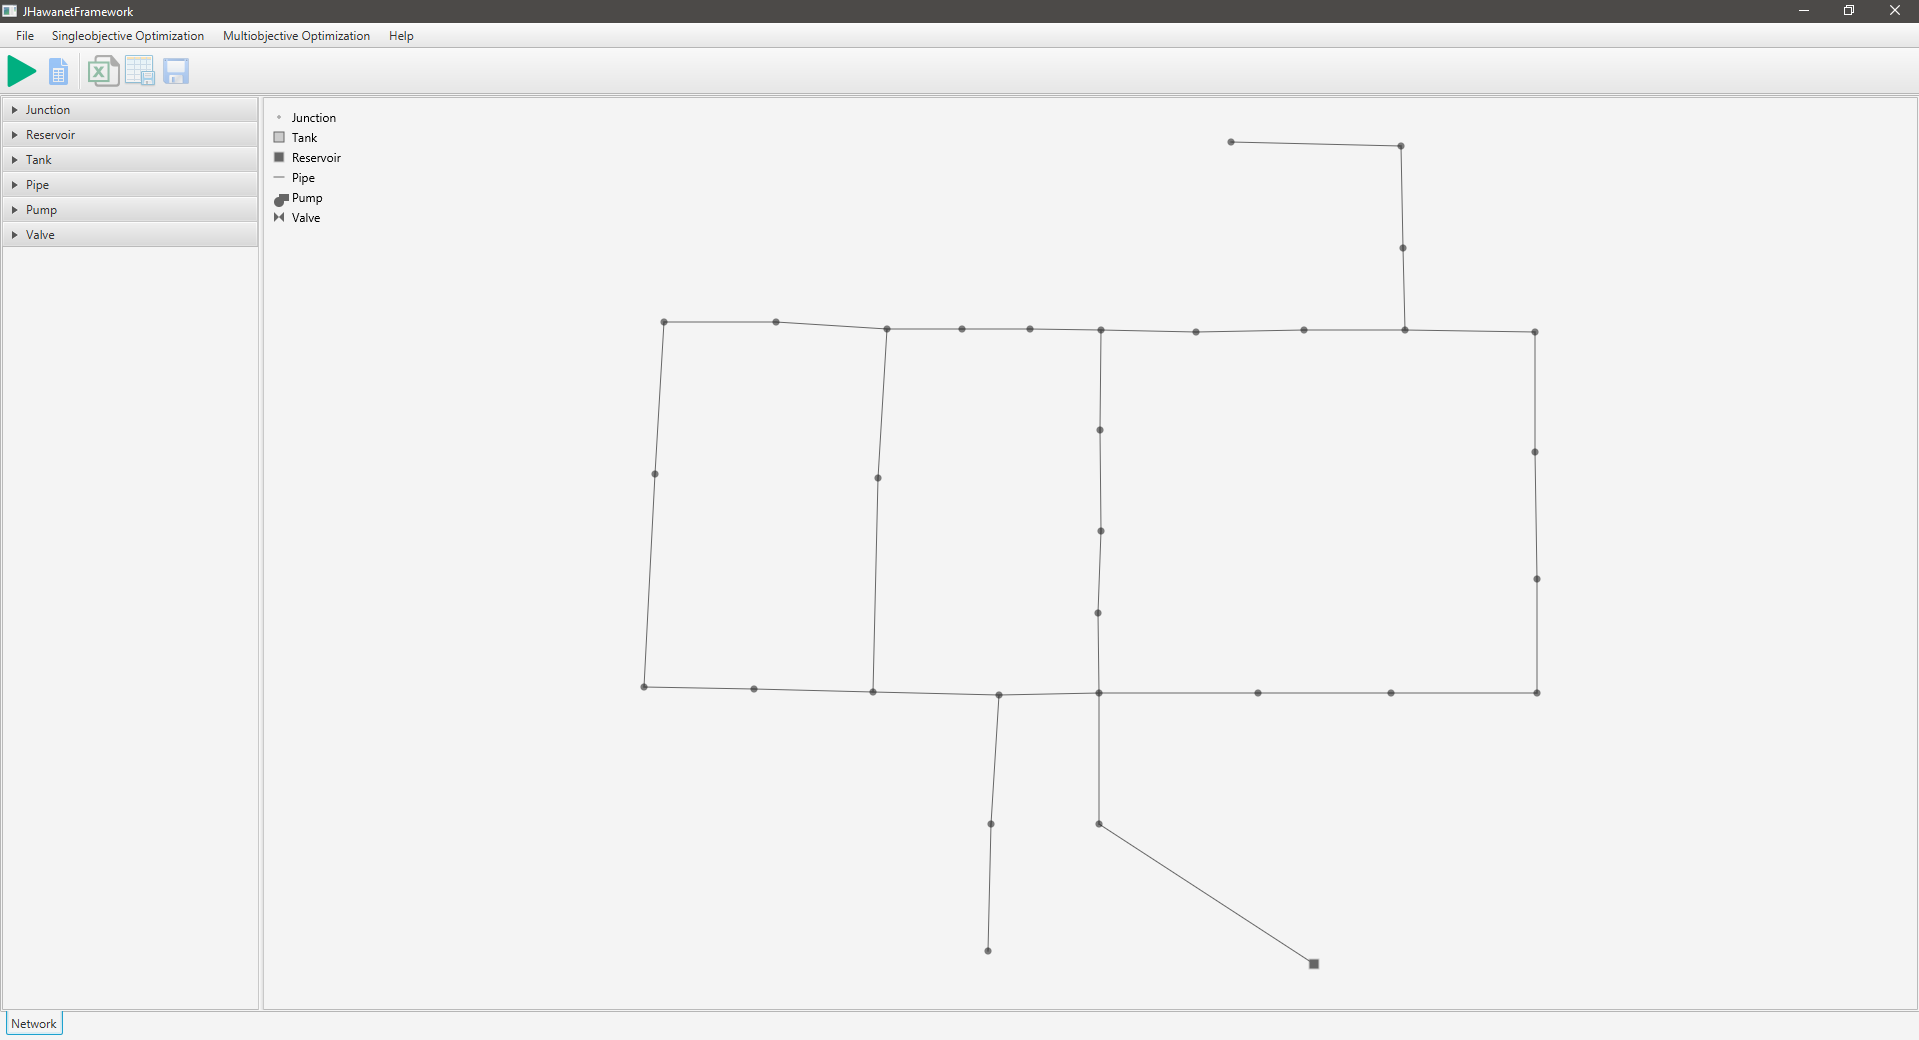
\includegraphics[width=\textwidth]{Capitulo4/assets/VisualizacionRed.png}
	\caption{Ventana principal de la aplicaci�n donde se visualiza la red}
	\label{fig:ventana_visualizacion}
\end{figure}

\paragraph{Funcionalidad 2}: Las Figuras~\ref{fig:ventana_descripcion},~\ref{fig:ventana_configuracion_problema},~\ref{fig:ventana_operador},~\ref{fig:ventana_retroalimentacion} y~\ref{fig:ventana_resultados_opt} muestran las ventana utilizadas durante el cumplimiento de esta funcionalidad.

\begin{figure}[H]
  \centering
  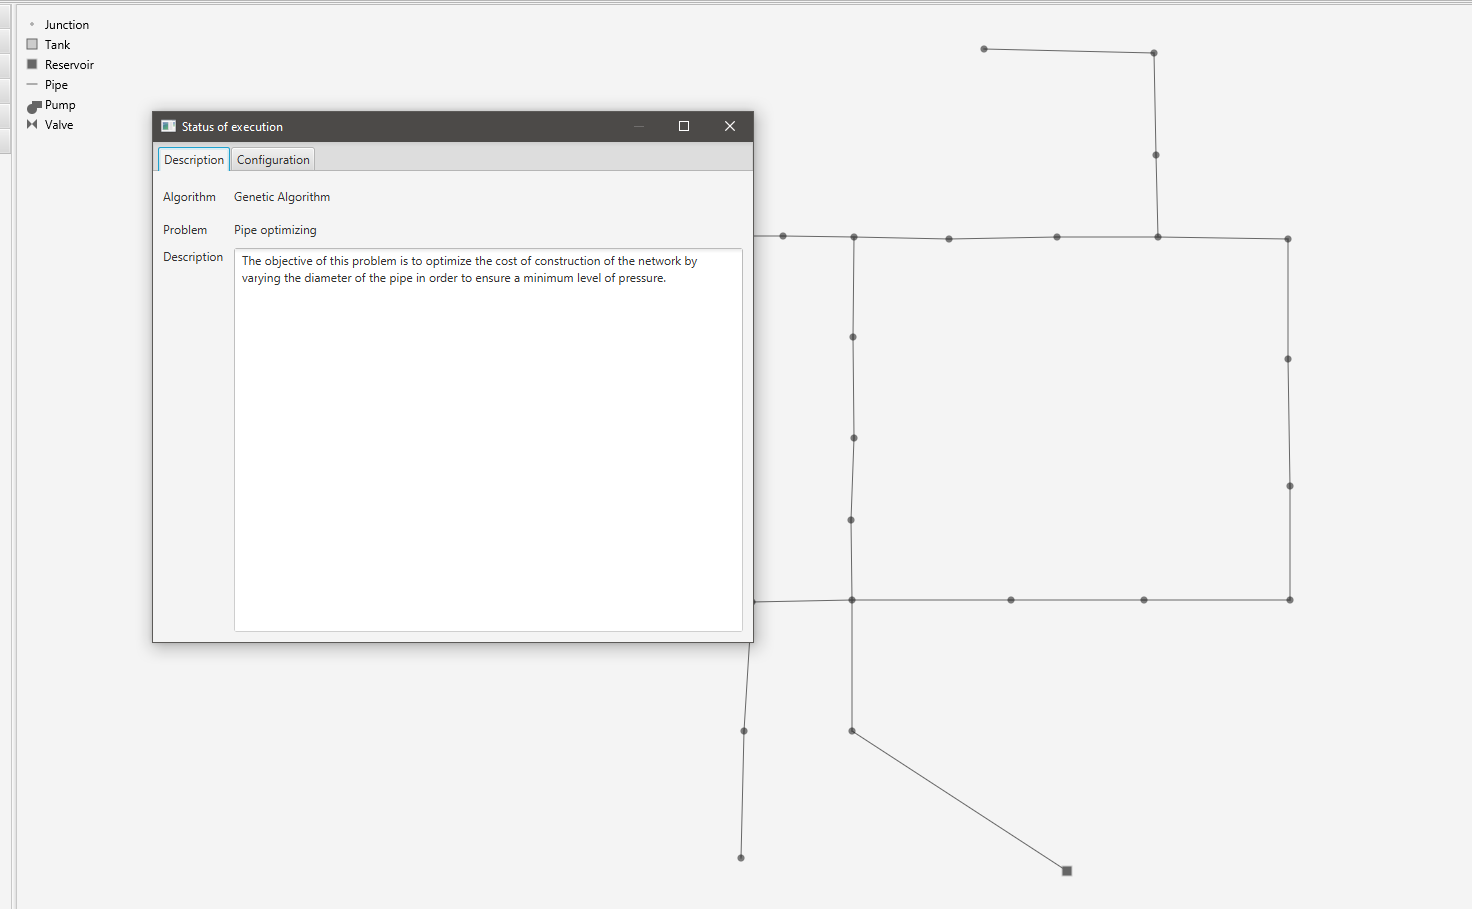
\includegraphics[width=\textwidth]{Capitulo4/assets/ConfiguracionProblema1.png}
	\caption{Ventana de descripci�n del problema.}
	\label{fig:ventana_descripcion}
\end{figure}

\begin{figure}[H]
  \centering
  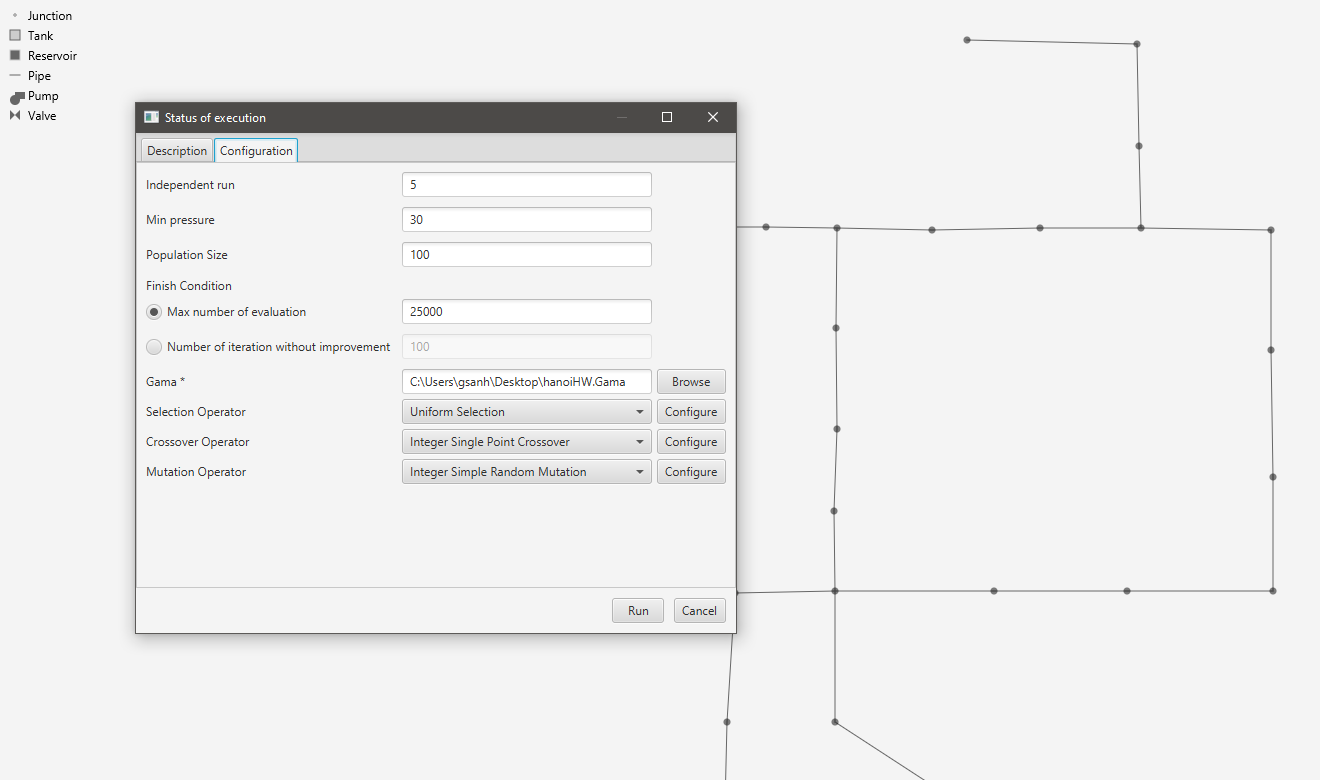
\includegraphics[width=\textwidth]{Capitulo4/assets/ConfiguracionProblema2.png}
	\caption{Ventana de configuraci�n del problema.}
	\label{fig:ventana_configuracion_problema}
\end{figure}

\begin{figure}[H]
  \centering
  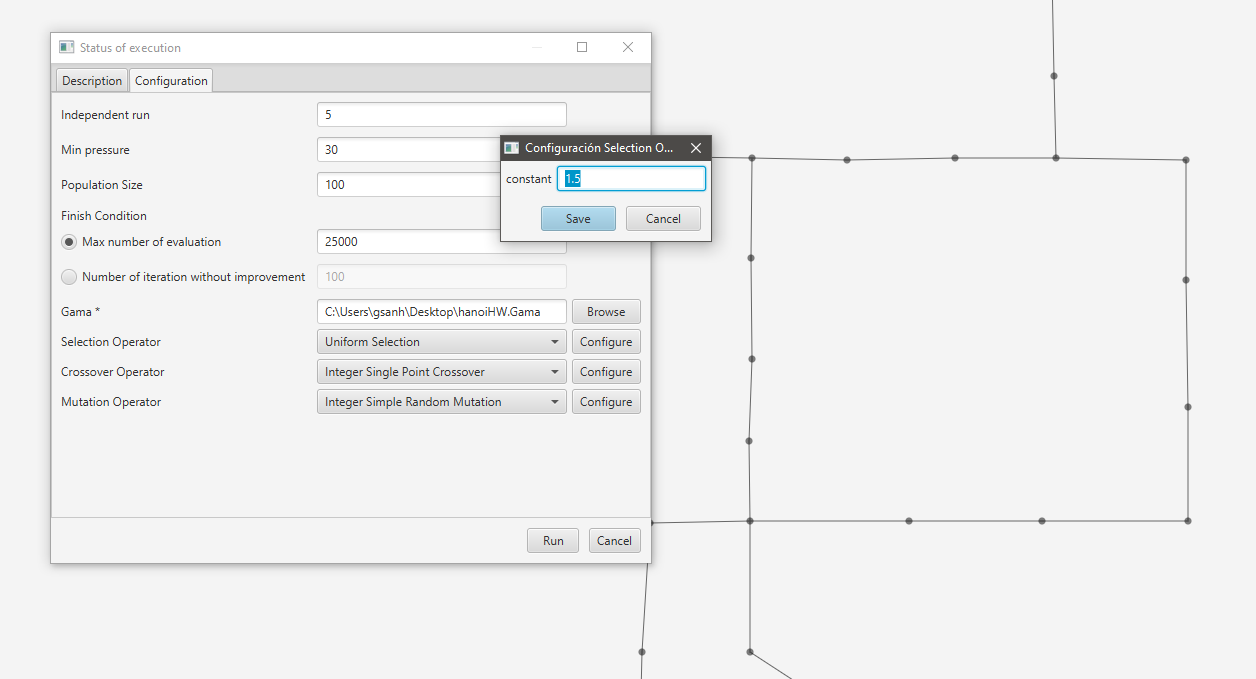
\includegraphics[width=\textwidth]{Capitulo4/assets/ConfiguracionProblema3.png}
	\caption{Ventana de configuraci�n de par�metros del operador \textit{UniformSelection}}
	\label{fig:ventana_operador}
\end{figure}

\begin{figure}[H]
  \centering
  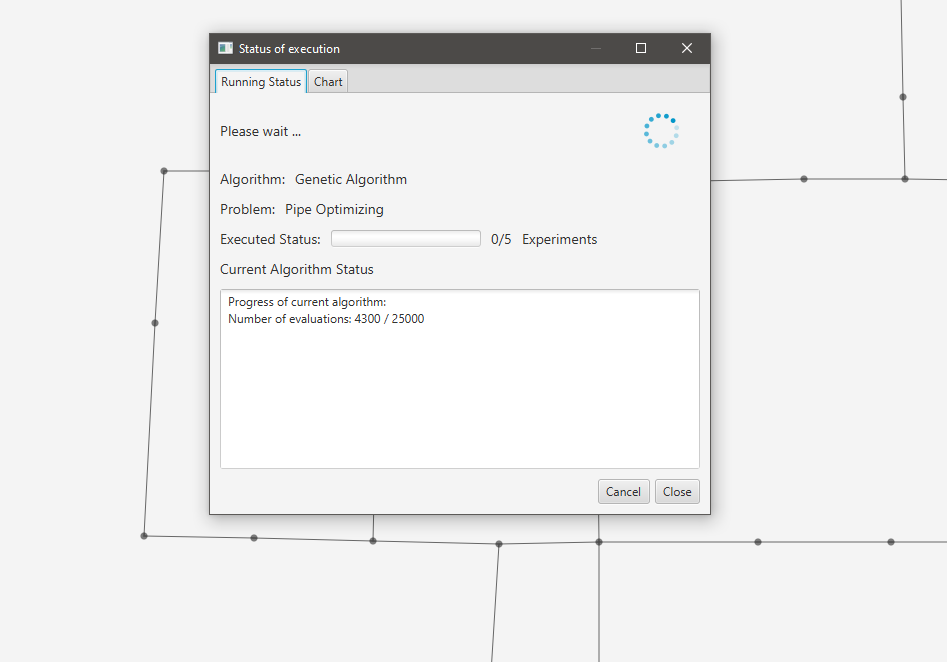
\includegraphics[width=\textwidth]{Capitulo4/assets/VentanaDeEjecucionMono.png}
	\caption{Ventana del retroalimentaci�n mostrada durante la ejecuci�n}
	\label{fig:ventana_retroalimentacion}
\end{figure}

\begin{figure}[H]
  \centering
  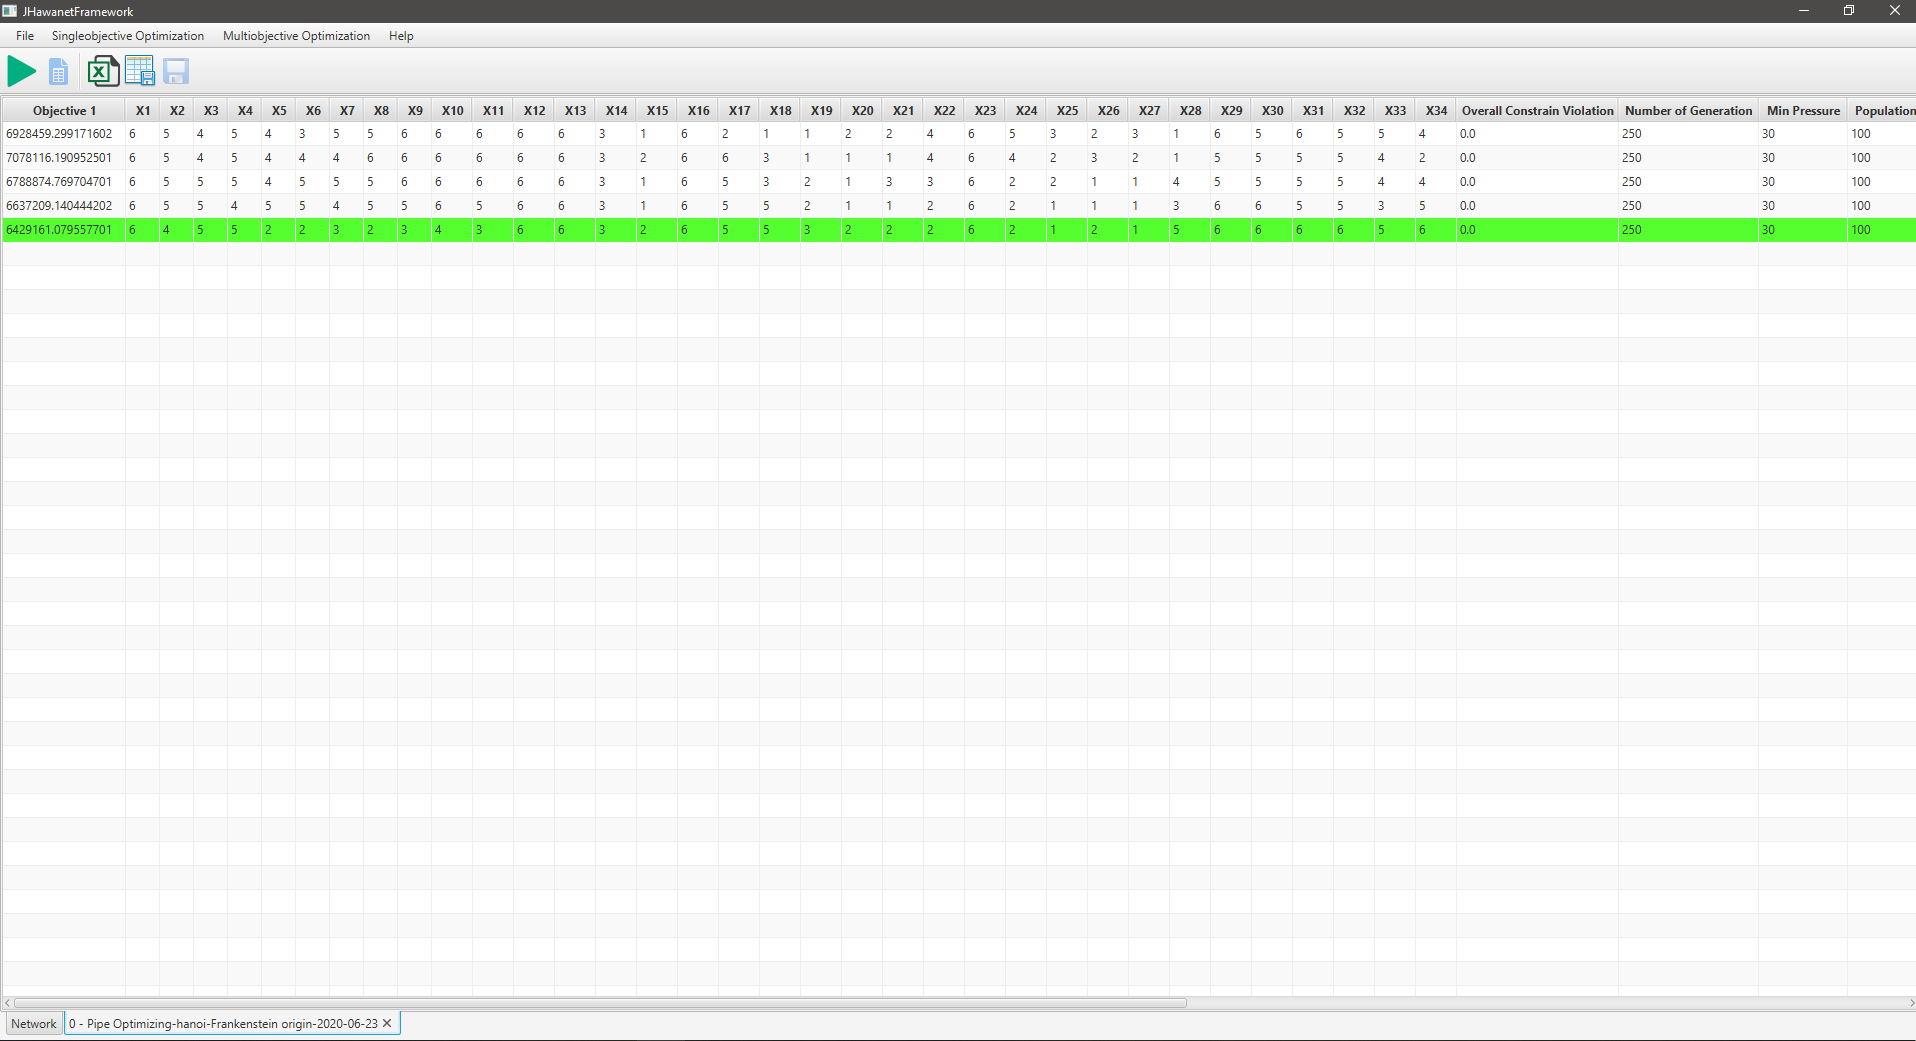
\includegraphics[width=\textwidth]{Capitulo4/assets/VentanaDeResultadosMono.png}
	\caption{Ventana de resultados generada cuando termina la ejecuci�n para el problema monoobjetivo Pipe Optimizing}
	\label{fig:ventana_resultados_opt}
\end{figure}

\paragraph{Funcionalidad 3}: La Figura~\ref{fig:ventana_simulacion_hyd} muestra la ventana con los resultados de una simulaci�n hidr�ulica para la red cargada.


\begin{figure}[H]
  \centering
  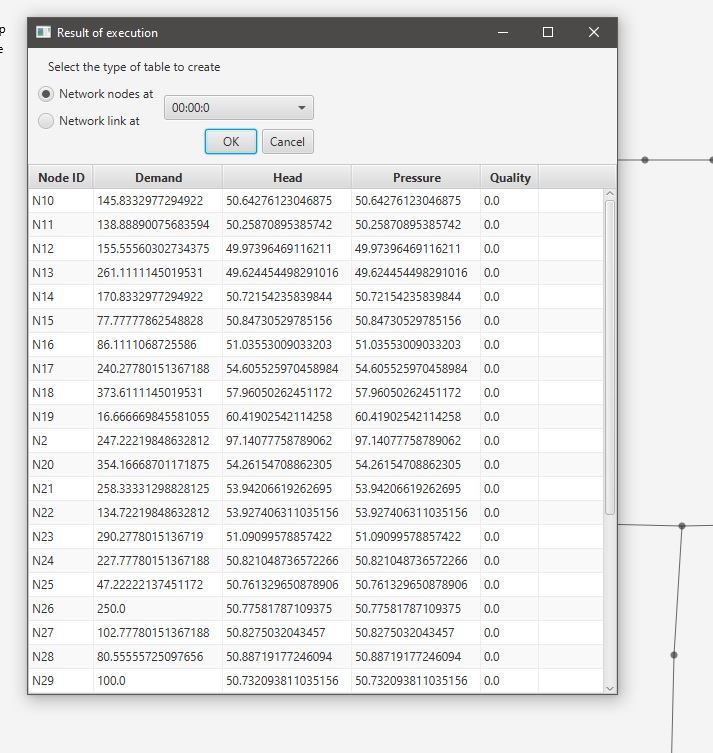
\includegraphics[width=\textwidth]{Capitulo4/assets/VentanaDeSimulacionHidraulica.png}
	\caption{Ventana de simulaci�n hidr�ulica utilizando los valores del archivo de red}
	\label{fig:ventana_simulacion_hyd}
\end{figure}

\subsection{Modelo matem�tico de los problemas}
En esta subsecci�n se presentan los modelos matem�ticos de los problemas resueltos, as� como la representaci�n de sus soluciones.

\subsubsection{\textit{Pipe Optimizing}}
\textit{Pipe Optimizing} es un problema de dise�o cuyo objetivo es minimizar el costo de inversi�n en la construcci�n de las tuber�as. Para �sto, se busca aquella combinaci�n de di�metros que disminuyan el costo de la construcci�n de las tuber�as a la vez que se cumplen las restricci�n de presi�n m�nima impuesta sobre la red. La ecuaci�n \ref{eq:costos_de_inversion} presentada en \cite{Pereyra2017} muestra la ecuaci�n a optimizar.
	
\begin{equation}
    \label{eq:costos_de_inversion}
    \begin{aligned}
        \text{Costo de inversi�n} = \sum_{i=1}^{N} (C_i \times D_i \times L_i)
    \end{aligned}
\end{equation}

En la ecuaci�n anteriormente presentada el termino $C_i$ se refiere al costo unitario de la tuber�a $i$, el t�rmino $D_i$ corresponde al di�metro de la tuber�a y finalmente $L_i$ hace referencia su longitud. Como se menciono anteriormente, el problema debe satisfacer la siguiente restricci�n:

\begin{equation}
    \label{eq:restriccion_costo_inversion}
    \begin{aligned}
        H_i < H_{min}
    \end{aligned}
\end{equation}

\noindent donde $H_i$ corresponde a la presi�n sobre la tuber�a $i$ y $H_{min}$ a la presi�n m�nima de la red.

La soluci�n retornada por el algoritmo utilizado, en este caso GA, se puede ver en la Figura~\ref{fig:solution_pipe_optimizing}. En dicha soluci�n los valores que toman la variable de decisi�n corresponden al �ndice a una tabla donde se encuentra el di�metro y el costo de la tuber�a. El largo de la tuber�a esta configurado en el archivo de configuraci�n de red (El archivo con extensi�n inp). 

\begin{figure}[H]
    \centering
    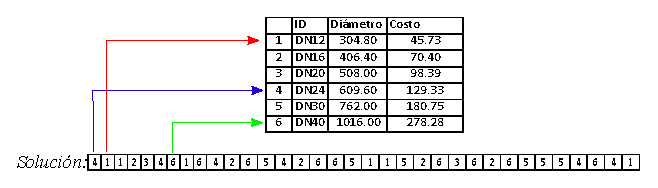
\includegraphics[width=\textwidth]{Capitulo4/assets/representacion_solucion_monoobjetivo.eps}
    \caption{Representaci�n de la soluci�n del problema monoobjetivo \textit{Pipe Optimizing}}
    \label{fig:solution_pipe_optimizing}
\end{figure}

\subsubsection{\textit{Pump Schedule}}

\textit{Pump Schedule} \cite{Makaremi2017, JHawanet-2019} es un problema de operaci�n que tiene como objetivos optimizar tanto el costo energ�tico, as� como el costo de operaci�n. A continuaci�n se expresan las ecuaciones utilizadas para calcular los objetivos y las restricciones.

Para el c�lculo de los costos energ�ticos se ocupa la siguiente ecuaci�n:
  
\begin{equation}
    \label{eq:costos_energeticos}
    \begin{aligned}
        C_E(S) &= \sum_{n=1}^{NP}\sum_{t=0}^{NT-1}(P_c(t) \times E_c(n, t) \times S(n, t))
    \end{aligned}
\end{equation}

\noindent donde:
\begin{itemize}
    \item	$C_E(S)$: Costos energ�tico.
    \item   $NP$: El numero de bombas.
    \item 	$NT$: N�mero de periodos de simulaci�n. El m�ximo son 24 horas.
    \item 	$P_c(t)$: La tarifa energ�tica en el periodo $t$.
    \item 	$E_c(n, t)$: Consumo energ�tico de la bomba $n$ en el tiempo $t$.
    \item 	$S(n,t)$: El estado de la bomba. 1 si esta encendida y 0 si esta apagada.
\end{itemize}

Para calcular el consumo energ�tico de la bomba $n$ se utiliza la siguiente formula:
\begin{equation}
    \label{eq:costos_energeticos}
    \begin{aligned}
        E_c(n, t) &= \frac{10^{-3} \times \gamma \times Q(n, t) \times h(n, t)}{e(n, t)}
    \end{aligned}
\end{equation}

\noindent donde:
\begin{itemize}
    \item	$\gamma$: Peso del agua.
    \item   $Q(n, t)$: Flujo a trav�s de la bomba $n$ en el tiempo $t$
    \item 	$h(n, t)$: Altura manom�trica de la bomba.
    \item 	$e(n, t)$: Eficiencia de la bomba $n$ en el tiempo $t$.
\end{itemize}

Para c�lcular el costo de bombeo se c�lcula el n�mero de encendido y apagados de todas las bombas en el periodo de tiempo analizado. Matem�ticamente la funci�n para calcular dicho costo corresponde a:

\begin{equation}
    \label{eq:costos_de_mantenimiento}
    \begin{aligned}
        C_N(S) &= \sum_{n=1}^{NP}\sum_{t=0}^{NT-1}r_t
    \end{aligned}
\end{equation}
donde:
\begin{itemize}
    \item $C_N(S)$ Costo de mantenimiento.
    \item $r_t$: Valor indicando si en el periodo $t$ hubo un cambio de estado en la bomba desde apagado a encendido. Este valor es 1 cuando la bomba ha sido encendida.
\end{itemize}

La funciones \ref{eq:costos_energeticos} y \ref{eq:costos_de_mantenimiento} deben cumplir las siguientes restricciones:
% restricciones asociadas a la conservaci�n de la masa y la energ�a; la presi�n m�nima, el caudal en la bomba $n$ y el nivel de agua almacenado en el reservorio en un periodo de tiempo especifico.

Conservaci�n de la masa:
\begin{equation}
    \label{eq:conservation_of_mass}
    \begin{aligned}
        \sum q_{in}-q_{out} &= C_j
    \end{aligned}
\end{equation}

\noindent donde:
\begin{itemize}
    \item $q_{in}$: Flujo de entrada.
    \item $q_{out}$: Flujo de salida.
    \item $C_j$: Consumo del nodo $j$.
\end{itemize}

Conservaci�n de la energ�a:
\begin{equation}
    \label{eq:conservation_of_energy}
    \begin{aligned}
        \sum h_f - \sum E_p &= 0
    \end{aligned}
\end{equation}

\noindent donde:
\begin{itemize}
    \item $h_f$: Perdida de energ�a por fricci�n.
    \item $E_p$: Energ�a aportada por la bomba.
\end{itemize}

Perdida de carga por fricci�n:
\begin{equation}
    \label{eq:pipe_head_losses}
    \begin{aligned}
        h_f &= \frac{10.67 \times L_q^{1.85}}{CH^{1.85} \times D^{4.87}}
    \end{aligned}
\end{equation}

\noindent donde:
\begin{itemize}
    \item $L_q$: Largo de la tuber�a.
    \item $CH$: Coeficiente de Hazen-Williams.
    \item $D$: Di�metro de la tuber�a.
\end{itemize}

Presi�n m�nima:
\begin{equation}
    \label{eq:min_pressure}
    \begin{aligned}
        H_i < H_{min}
    \end{aligned}
\end{equation}

\noindent donde:
\begin{itemize}
    \item $H_i$: Presi�n en el nodo $i$.
    \item $H_{min}$: Presi�n m�nima.
\end{itemize}

Caudal:
\begin{equation}
    \label{eq:min_pressure}
    \begin{aligned}
        Q_{i,t} \geq Q_i^{max}
    \end{aligned}
\end{equation}

\noindent donde:
\begin{itemize}
    \item $Q_{i,t}$: Caudal del nodo $i$ en el tiempo $t$.
    \item $Q_i^{max}$: Caudal m�ximo del nodo $i$.
\end{itemize}

Nivel de dep�sito:
\begin{equation}
    \label{eq:min_pressure}
    \begin{aligned}
        TS_{i, NT} \geq TS_{i, 0}
    \end{aligned}
\end{equation}

\noindent donde:
\begin{itemize}
    \item $TS_{i, NT}$: Nivel del reservorio $i$ en el tiempo $t$.
    \item $TS_{i, 0}$: Nivel del reservorio $i$ en el tiempo $0$.
\end{itemize}

En la Figura~\ref{fig:solution_pump_schedule} muestra como se codifica la soluci�n a este problema. Como se puede observar la soluci�n cuenta con 24 variables de decisi�n correspondiente a las 24 horas del d�a. Cada variable es un �ndice a la matriz de combinaciones posibles para cada bomba. Posteriormente, se genera una matriz binaria en donde cada fila es una bomba, cada columna es el periodo y el valor es el estado de la bomba en dicho periodo. Esta matriz binaria es usada para calcular el n�mero de cambios de estado en las bombas de la ecuaci�n \ref{eq:costos_de_mantenimiento}, asi como para obtener el estado de la bomba en el periodo $t$ de la ecuaci�n \ref{eq:costos_energeticos} referente al termino $S(n, t)$.

\begin{figure}[H]
    \centering
    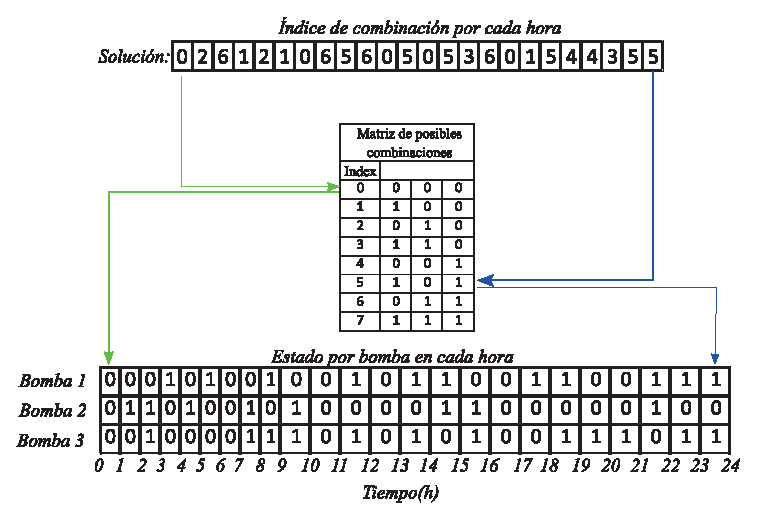
\includegraphics[width=\textwidth]{Capitulo4/assets/representacion_solucion_multiobjetivo.eps}
    \caption{Representaci�n de la soluci�n problema multiobjetivo \textit{Pump Schedule}}
    \label{fig:solution_pump_schedule}
  \end{figure}
